\documentclass{article}

\usepackage[english]{babel}
\usepackage{amsthm}
\usepackage{amsmath}
\usepackage{amssymb}
\usepackage{xcolor}
\usepackage{graphicx}
\usepackage{geometry}
\geometry{
    a4paper,
    total={170mm,257mm},
    left=20mm,
    top=20mm,
}
\usepackage{hyperref}
% \hypersetup{
%     colorlinks=true,
%     linkcolor=blue,
%     filecolor=magenta,      
%     urlcolor=cyan,
%     pdftitle={Overleaf Example},
%     pdfpagemode=FullScreen,
% }

\usepackage{cleveref}


\graphicspath{{./images/}}

\theoremstyle{definition}
\newtheorem{definition}{Definition}[section]

\newtheorem{theorem}{Theorem}[section]
\newtheorem{lemma}[theorem]{Lemma}
\newtheorem{proposition}[theorem]{Proposition}
\newcommand{\blue}[1]{\textcolor{blue}{#1}}

\title{Special Properties of Gradient Descent with Large Learning Rates}
\author{Denis Grachev}

\begin{document}
\maketitle

\begin{abstract}
This article is an overview of the work \cite{mohtashami2023special}
with some additional experiments. 
It has been widely observed that usage of larger learning 
rate in stochastic gradient descent often results into better models.
However theoretical reasons for this phenomena are not well understood yet.
Previous studies linked it to stochastic noise in SGD. 
The work focuses on theoretical proof of escaping local minima 
for some special class of functions. 
Also it is shown that for certain starting points and loss functions
GD with large learning rate has different trajectory 
and may lead to convergence to another minima, 
which is likely to be more robust. 

\end{abstract}

% \section{Introduction}

\section{Main results}
Usage of large learning rate is often explained by intuition of 
escaping local minima. 
In this work a class $C_l$ of functions is constructed 
which have at least two minima ($x^\dagger$ and $x_\ast$) and 
with a large learning rate GD with random initialization converges 
to $x_\ast$ almost surely, but with smaller learning rate 
there is strictly positive probability of converging to $x^\dagger$.

\section{Theoretical Analysis}
For analysis optimization problem using full-batch
gradient descent with random initialization was taken:
$$ f_* := \min_{x \in \mathbb{R}^d} f(x).$$
$f$ is supposed to be $L$-smooth over regions of the landscape 
so that the gradient does not change too sharply. 
Also we would require sharpness of some regions of $f$ 
around local minima using 
$\mu$-one-point-strongly-convexity (OPSC) with respect to $x_\ast$ over $M$.

\begin{definition}[$L$-smoothness]
    A function $f: \mathbb{R}^d \rightarrow \mathbb{R}$ 
    is $L$-smooth if $f$ is differentiable and 
    exists $L: \| \nabla f(x) - \nabla f(y)\| \leq L \| x - y \|, \: \forall x, y \in \mathbb{R}^d$ 
\end{definition}

\begin{definition}[$\mu$-one-point-strongly-convex (OPSC) with respect to $x_\ast$ over $M$]
    A function $f: \mathbb{R}^d \rightarrow \mathbb{R}$ is 
    $\mu$-one-point-strongly-convex (OPSC) with respect to $x_\ast$ over $M$ 
    if it is differentiable and 
    $$\exists \mu > 0: \langle \nabla f(x), x - x_\ast \rangle \geq \mu \| x - x_\ast\|^2, \: \forall x \in M.$$
\end{definition}

\begin{lemma}\label{lma1}
    Let $f$ be a function that is 
    $L_{\mathrm{global}}$ -smooth with a global minimum $x_\ast$. 
    Assume there exists a local minimum $x^\dagger$ around which
    \begin{itemize}
        \item $f$ is $\mu^\dagger$-OPSC woth respect to 
        $x^\dagger$ over a set $M$ that contains $x^\dagger$ with diameter $r$.
        
        \item Let $P(M)$ be a ball around $x^\dagger$ with radius 
        $r_P$ excluding points M. $f$ is 
        $L < L_{\mathrm{global}}$ -smooth in $P(M)$ and 
        $\mu_\ast$-OPSC with respect to $x_\ast$, 
        such as $\mu^\dagger > \frac{2L^2}{\mu_\ast}$. 
        $r_P$ depends on $r, \gamma, L_{\mathrm{global}}$.

        \item $\| x_\ast - x^\dagger \| > \tau$, where $\tau$ depends on $\mu_\ast, r, \gamma$. 

        Then using learning rate $\frac{2}{\mu^\dagger} < \gamma < \frac{\mu_\ast}{L^2}$
        GD escape $M$ and reach a point closer to $x_\ast$ than 
        $\| x^\dagger - x_\ast\| - r$ almost surely. 

    \end{itemize}
\end{lemma}
\begin{proof}
    
\end{proof}

\begin{figure}[h]
    \caption{Illustation of regions from \cref{lma1}}
    \label{fig:func}
    \centering
    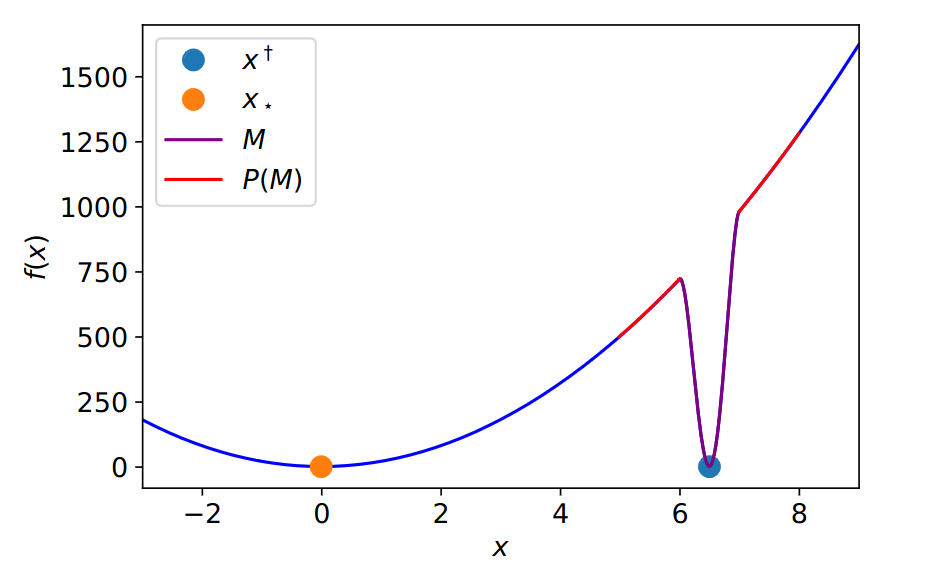
\includegraphics[scale=0.2]{lemma1}
\end{figure}

\begin{theorem}\label{thm1}
    Let $C_l$ be the set of functions sudh as $f$ is 
    $L$-smooth and $\mu_\ast$-OPSC with respect to the 
    global minima $x_\ast$ except n a region $M$ that 
    contains local minima $x^\dagger$ and satisfies \cref{lma1}.
    \begin{itemize}
        \item Gradient descent initialized randomly inside $M$ 
        with learning rate $\gamma < \frac{\mu^\dagger}{L^2_{\mathrm{global}}}$
        converges to $x^\dagger$ almost surely.
        
        \item Gradient descent initialized randomly in 
        arbitrary set $W: \mathcal{L}(W) > 0$ 
        with learning rate $\frac{2}{\mu^\dagger} < gamma \leq \frac{\mu_\ast}{L^2}$
        converges to $x_\ast$ almost surely.

    \end{itemize} 

\end{theorem}
\begin{proof}
    
\end{proof}

\begin{lemma}\label{lma2}
    Take gradient descent initialized randomly in set $W$ 
    with learning rate $\gamma \leq \frac{1}{2L}$.
    Let $X \subset \mathbb{R}^d$ arbitrary set of points in 
    the landscape, $f$ is $L$-smooth over 
    $\mathbb{R}^d \setminus X$. Probabilty of encountering 
    any point of $X$ in first $T$ steps of gradient descent is 
    at most $2 ^ {(T + 1)d} \frac{\mathcal{L}(X)}{\mathcal{L}(W)}$.
\end{lemma}
\begin{proof}
    
\end{proof}

\begin{theorem}\label{thm2}
    Let $X$ be an arbitrary set of points, 
    $f$ is $\mu_\ast$-OPSC with respect to a minima 
    $x_\ast \notin X$ over $\mathbb{R}^d \setminus X$.
    Let $c_X := \inf \left\{ \| x - x_\ast \| \:|\: x \in X  \right\}$
    and $r_W := \sup \left\{ \| x - x_\ast \| \:|\: x \in W \right\}$.
    The probability of not encountering ant points of $X$ during 
    gradient descent with learning rate $\gamma \leq \frac{\mu_\ast}{L^2}$
    is at least $1 - \frac{r_W}{c_X}^{\frac{-d}{\log_2(1 - \gamma \mu_\ast)}} \frac{\mathcal{L}(X)}{\mathcal{L}(W)} 2^d$
    if $c_X \leq r_W$ and $1$ otherwise.
\end{theorem}

\begin{proof}
    
\end{proof}

\section*{Proposition}
Take the case of SGD 
$$ 
x_{t + 1} := x_t - \gamma \left( 
    \nabla f(x_t) + \xi_t
\right),
$$
where $\xi_t$ considered to be $\mathrm{Uniform}(-\sigma, \sigma)$.

\begin{proposition}
    Consider SGD on the function from figure \ref{fig:func}, 
    starting close to $x^\dagger$.
    If the learning rate is sufficiently small the iterations
    will never converge to $x_\ast$ nor to a small region around it, 
    regardless of the magnitude of the noise. 
    If the learning rate is large enough and stochastic noise
    satisfies certain bounds, SGD will converge to $x_\ast$ 
    from any starting point.
\end{proposition}

\begin{proof}
    
\end{proof}

\clearpage 

\section{Experiments}
\subsection*{1D Example}
Study different GD behaviour depending on starting point and learning rate 
on the function $f$. 
$$
f(x):= \begin{cases}
    -1600(x-2.5)^5-2000(x-2.5)^4+800(x-2.5)^3+1020(x-2.5)^2 & 2 \leq x \leq 3 \\ 
    1411.2 \times\left(1-10^4(x-8.4)\right) & 8.4 \leq x \leq 8.40001 \\ 
    0 & 8.40001 \leq x \leq 8.59999, \\ 
    1479.2 \times\left(10^4(x-8.6)+1\right) & 8.59999 \leq x \leq 8.6, \\ 
    20 x^2 & \textit{ otherwise }
\end{cases}
$$

\begin{figure}[!htb]
    \caption{Visual comparison of GD with different learning rates.}
    \minipage{0.33\textwidth}
      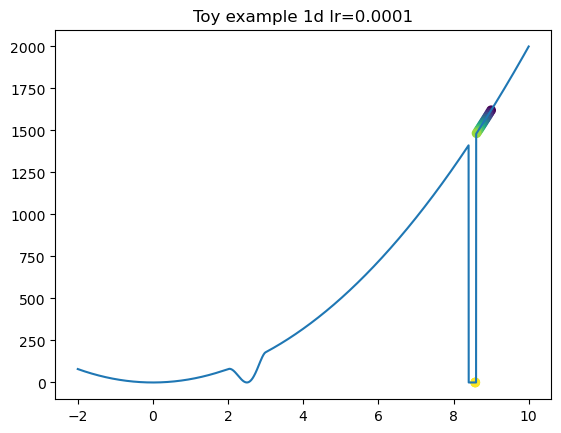
\includegraphics[width=\linewidth]{1d_example_min_near_start.png}
      \caption{GD converged to local minima close to start.}
    \endminipage\hfill
    \minipage{0.32\textwidth}
      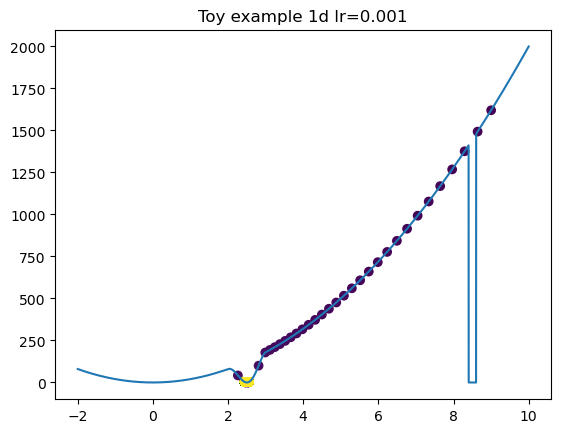
\includegraphics[width=\linewidth]{1d_example_local_min.png}
      \caption{GD converged to local minima.}
    \endminipage\hfill
    \minipage{0.32\textwidth}%
      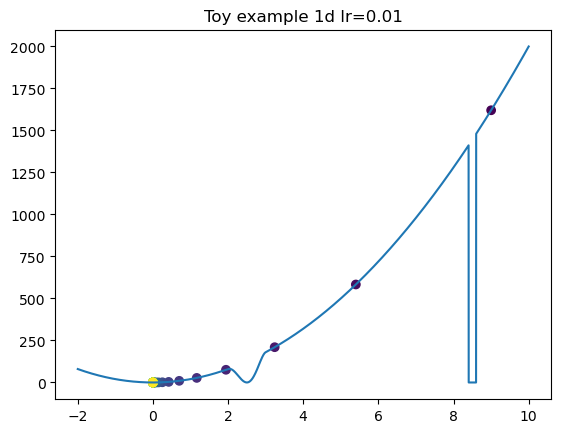
\includegraphics[width=\linewidth]{1d_example_global_min.png}
      \caption{GD converged to global minima.}
    \endminipage
\end{figure}

\begin{figure}[!htb]
    \begin{center}
        \caption{Types of convegence of GD depending on startpoint and learning rate.}
        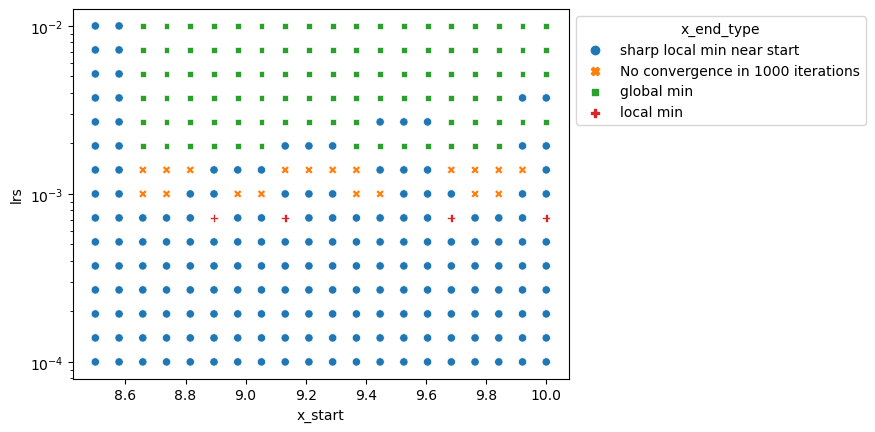
\includegraphics[scale=0.7]{1d_learning_rate_stats.png}        
    \end{center}
\end{figure}

From the experiments we can see that usage of larger learning rates
helps to escape local minima and converge to a flatter one.

\clearpage

\subsection{2D Example}
Study different GD behaviour depending on learning rate on
the function $f$

$$
f(x, y):=x^2+y^2-200 \mathrm{ReLU}(|x|-1) \mathrm{ReLU}(|y|-1) \mathrm{ReLU}(2-|x|) \mathrm{ReLU}(2-|x|)
$$


\begin{figure}[h]
    \caption{Visual comparison of GD with different learning rates.}
    \minipage{0.48\textwidth}
      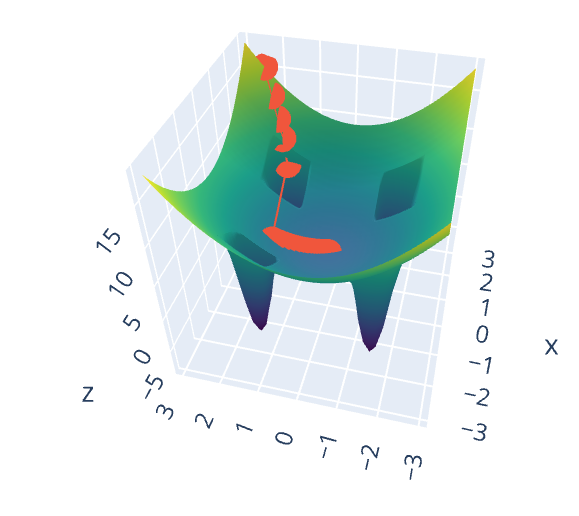
\includegraphics[width=\linewidth]{2d_example_flat.png}
      \caption{GD converged to flat minima.}
    \endminipage\hfill
    \minipage{0.48\textwidth}
      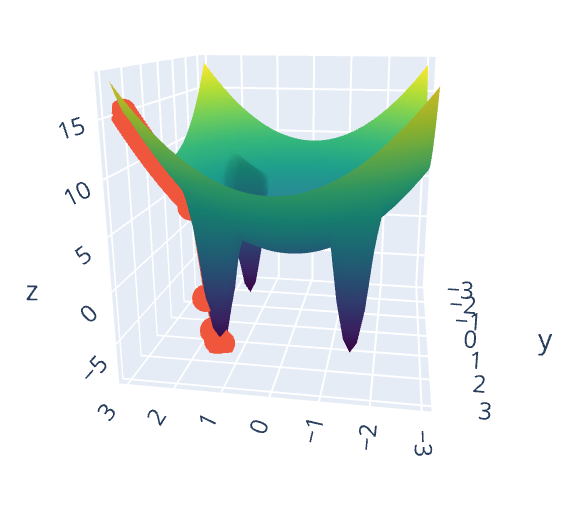
\includegraphics[width=\linewidth]{2d_example_sharp.png}
      \caption{GD converged to sharp minima.}
    \endminipage
\end{figure}

\begin{figure}[h]
    \begin{center}
        \caption{Share of GDs that obtained flat minima if starting point is random $3 \leq x, y \leq 4$.}
        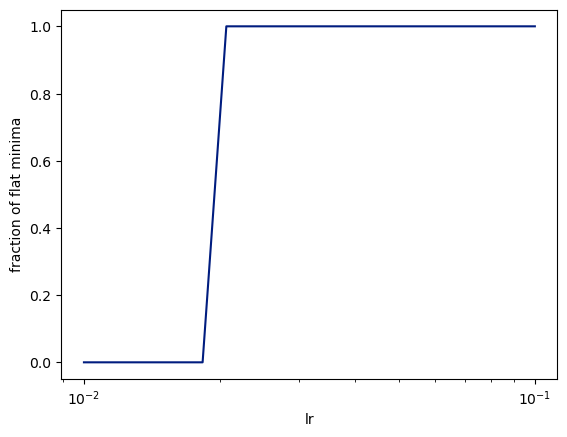
\includegraphics[scale=0.7]{2d_example_lr_vs_minima.png}        
    \end{center}
\end{figure}

\subsection{MNIST example}
Not yet finished experiments
\begin{itemize}
    \item Warm up NN using small learning rate.
    Use large and small learning rate,
    according to figure 7 from \cite{mohtashami2023special} 
    they might have different trajectories and converge to 
    different minima. 

    \item Test hypothesis that minima obtained using larger 
    learning rate is more robust. 
    Train NN using large and small learning rate.
    Then change the training dataset and continue to train.
    Compare distance between minima of different datasets 
    obtained small and large learning rate.  

\end{itemize}

\bibliographystyle{alpha}
\bibliography{sample}

\end{document}
